% "Compositing shaders in X3D" by Michalis Kamburelis,
% for Web3D 2011.
%
% If accepted, this will be © Copyright 2011 by ACM, Inc.
% See http://www.acm.org/publications/policies/copyright_policy
%

%% Template stuff begins here ------------------------------------------------

\documentclass{acmsiggraph}                     % final
%\documentclass[annualconference]{acmsiggraph}  % final (annual conference)
%\documentclass[review]{acmsiggraph}            % review
%\documentclass[widereview]{acmsiggraph}        % wide-spaced review
%\documentclass[preprint]{acmsiggraph}          % preprint

\usepackage[scaled=.92]{helvet}
\usepackage{times}
\usepackage{graphicx}
\usepackage{parskip}
\usepackage[labelfont=bf,textfont=it]{caption}
\onlineid{1010} %% I think this doesn't matter

%% Template stuff ends here ------------------------------------------------

% This is really the only sensible way to make breaking of monospace text
% (everything inside \texttt, including (but not limited) to urls).
% Otherwise, the monospace text flows outside of the column all over the place.
\sloppy

\usepackage{needspace}

%% For href
\usepackage{ifpdf}
\ifpdf
  \usepackage[pdftex]{hyperref}
\else
  \usepackage[hypertex]{hyperref}
\fi

%% Put float in a nice box,
%% http://en.wikibooks.org/wiki/LaTeX/Floats,_Figures_and_Captions
\usepackage{float}
\floatstyle{boxed}
\newfloat{mycodecore}{H}{listofmycode}
\floatname{mycodecore}{}

% Fix mycodecore: it has additional vertical line at the bottom after the frame.
% Possibly due to Verbatim inside?
\newenvironment{mycode}
{\begin{mycodecore}}
{\end{mycodecore}
\vspace{-0.1in}}

%% Use verbatim that allows \latex commands inside,
%% highly useful for my node spec figures.
%% See http://scott.sherrillmix.com/blog/category/programmer/latex/,
%% http://www.ctan.org/tex-archive/macros/latex/contrib/fancyvrb/
\usepackage{fancyvrb}

%% To allow tex_projected at the bottom.
%% Without this, figure* can only go to the top (or separate page).
%% http://en.wikibooks.org/wiki/LaTeX/Floats,_Figures_and_Captions#Wide_figures_in_two_column_documents
\usepackage{stfloats}

%% Bold inside our code/spec samples.
\newcommand*{\codeem}[1]{\textbf{#1}}

% \nolinkurl is a trick to allow links to break across lines in pdf,
% from http://www.miwie.org/tex-refs/html/latex-packages.html#hyperref
\newcommand*{\myhref}[2]{\texttt{\href{#1}{\nolinkurl{#2}}}}

% The above \myhref unfortunately (due to \nolinkurl trick)
% makes it impossible to break links manually.
% So below is the same as \myhref, but does not break link text automatically,
% and allows to break it manually (by inserting \\ etc.)
% \newcommand*{\myhrefm}[2]{\texttt{\href{#1}{#2}}}

\newenvironment{myenumerate}
{\begin{enumerate}
  \setlength{\itemsep}{0pt}
  \setlength{\parskip}{0pt}
  \setlength{\parsep}{0pt}}
{\end{enumerate}}

\title{Compositing shaders in X3D}

\author{Michalis Kamburelis\thanks{e-mail: michalis.kambi@gmail.com}\\Institute of Computer Science\\University of Wroc{\l}aw, Poland}

\keywords{X3D graphics, shaders, GLSL, shadows, shadow maps, bump mapping}

\begin{document}

\teaser{
  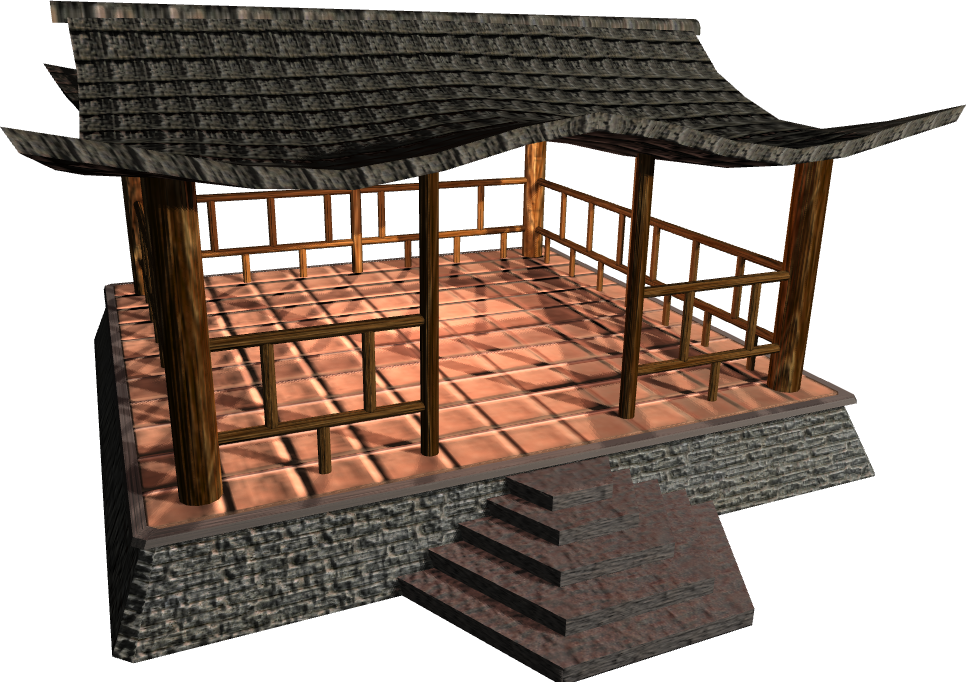
\includegraphics[width=2.19in]{rhan_shrine_5_everything}
  \caption{Bump mapping and 2 shadow maps on the same shape.}
}

\maketitle

\begin{abstract}
We demonstrate a flexible way to implement effects in X3D \cite{x3d:spec}
by shader programming.
Our approach allows to define the effects at appropriate places
(not only at Appearance, but also at particular light sources, texture and such).
It allows to seamlessly combine many effects, defined by X3D author,
with the shader defined internally by X3D browser.
Thus, it makes designing new effects in the GPU shading language trivial,
both for the browser implementors and for X3D authors. Various effects
cooperate automatically, and may be trivially composed by the X3D author.
And it still allows to design effects using the full power of GPU shading
language. We deliberately do not invent a new language, thus allowing
the authors the use all the shading language features for given GPU,
and allowing for easy implementation --- there is no need for any complex
language processing inside X3D browser.
\end{abstract}

\begin{CRcatlist}
%% TODO: update it
  \CRcat{I.3.7}{Computer Graphics}{Three-Dimensional Graphics and Realism}{Color, shading, shadowing, and texture};
  \CRcat{I.3.6}{Computer Graphics}{Methodology and Techniques}{Languages, Standards}
\end{CRcatlist}

\keywordlist

%% \terms{Languages, Standardization, Algorithms}
%% not needed with acmsiggraph template?

\section{Introduction}

%% The ``\copyrightspace'' command must be the first command after the
%% start of the first section of the body of your paper. It ensures the
%% copyright space is left at the bottom of the first column on the first
%% page of your paper.
\copyrightspace

We present a technique for composing many shader snippets into a
single shader code. X3D browsers can use it to allow user and browser
shaders to coexist. Thus, users benefit from all the effects
implemented in the browser, even when they want to add some effect by
explicit shader code. Users can also seamlessly connect various
effects into a shape, without the need to adjust any shader source
code. Even the browser's implementation can be simplified, by using
the same mechanism to separate implementation of various effects
within a browser.

For an interesting example, consider three effects: shadows, bump
mapping, and lighting equations. Shadows provide an information that
either turns on or off a particular lighting contribution (or scales
this contribution, in case of soft shadows). Lighting equation
calculates light contribution, looking at material, light source and
normal at given geometry point. Bump mapping
\cite{vrmleng:bumpmapping} (in the simplest case)
modifies how the normal value is obtained: when bump mapping is used,
the normal is taken from the texture. So we have

$$ shadow(light) * light\_contribution(light, material, normal(point)) $$

In case of no shadows, shadow(x) = 1. In case of no bump mapping,
normal is determined by the geometry (per-face, or smoothed per-face),
and usually is passed as an already calculated attribute to the
shader. We would like to be able to modify these three functions independently.

\section{Motivation and previous work}

Current shading description methods do not allow easy connecting
many effects into a single shader.

Shading source code files (GLSL, Cg) make no such way.

Effects formats (HLSL .fx, CgFX) allows to choose one technique, and
within it make passes. No way of automatically connecting one .fx file
with another.

One oldest solution: make a library of functions (like GLSL
functions), and allow to user to use them. But this is very bad and
limited. You cannot e.g. insert a shadow check right before adding the
light contribution (and still use browser code outside (to iterate
over lights) and inside (to calculate single light contribution)).

Another common solution is to arrange shaders in a pipe, where one
shader processes the result of another. This can be visualized as
layers of materials, where each layer modifies the previous
layer. However, this is again not flexible --- there's no way to plug
in your code in the middle of another shader's work.

An older solution, in the spirit of above, was also to perform
multi-pass rendering. However, this (in addition to lack of
flexibility of previous approach) makes also a loss of rendering
speed. In our work, we want to allow a single rendering pass to be as
powerful as it can.

%% (see also http://groups.google.com/group/blendertorenderman/browse_thread/thread/aaf07831b91be9db?pli=1 , confirms my findings)

Another approach is the Sh (ref:http://libsh.org/) language, which
allows writing shaders code (that can run on GPU) directly inside a
C++ program. For this, Sh extends the C++ language (through C++
operator overloading and macros tricks). It allows an excellent
integration between C++ code and shaders, hiding the ugly details of
passing variables between normal code (that executes on CPU) and
shader code (that usually executes on GPU). You can use
object-oriented methods there to create a general shader that can
later be extended through various means, like overriding virtual
methods. However, this is a solution closely coupled with C++. It's
suitable if you have a 3D engine in C++, and you want to use in your
own C++ program and extend it's shaders. In this paper, we want to
create a solution that is absolutely separate from the programming
language used to make a browser. Invoking a compiler to generate a
final GPU shader, not to mention teaching user's C++, is out of the
question.

%% ("Metaprogramming GPUs with Sh", http://books.google.com/books?id=8RX4RmFRLmgC&pg=PA79&lpg=PA79&dq=ShAttrib2f&source=bl&ots=IOxd1-BQLL&sig=AIPgFRmbodNpCLWmwk-QV5JUjVo&hl=pl&ei=EylRTe7RB8qeOsiQ1aQI&sa=X&oi=book_result&ct=result&resnum=7&ved=0CEkQ6AEwBg#v=onepage&q=ShAttrib2f&f=false )

At the end, we would like to mention a solution from a completely
different domain, that is surprisingly similar to ours in some ways.
Drupal, an open-source CMS system written in PHP,
has a very nice system of modules. Each module
can extend the functionality of the base system (or other module)
by implementing a \textit{hook}, which is just a normal PHP function
with a special name and appropriate set of parameters. Modules can also define
their own hooks (for use by other modules) and invoke them when appropriate.
This creates a system where it's trivially easy to define a hook,
and to use a hook.
Many modules can implement the same hook and cooperate without any problems.
The whole hook system is defined completely in PHP, as it's a scripting
language, and you can query the list of loaded functions by name,
and call function by name.

This is actually quite similar to our base idea of combining effects
inside Appearance.effects field. Our effects are similar to
Drupal's modules, as our ,,plugging points'' are analgous to Drupal hooks.
Our effects can define functions with special names to override
standard shader behavior. They can also define new names of plugs, for other
effects to use. Of course we also have some special problems
(shading language is quite far from a scripting language,
so defining hooks is done by smart textual replacements)
and some special opportunities (we can define effects at
the appropriate nodes of X3D, like textures and lights sources,
as we don't want to throw all the effects in one bag).

\begin{figure*}[t]
  \centering
  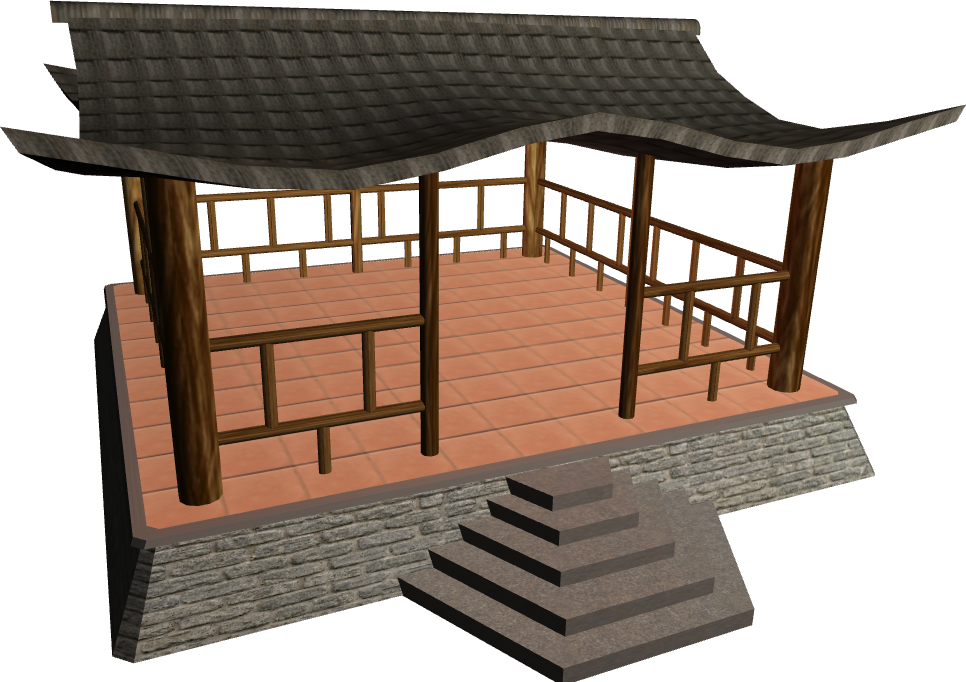
\includegraphics[width=2.2in]{rhan_shrine_0}
  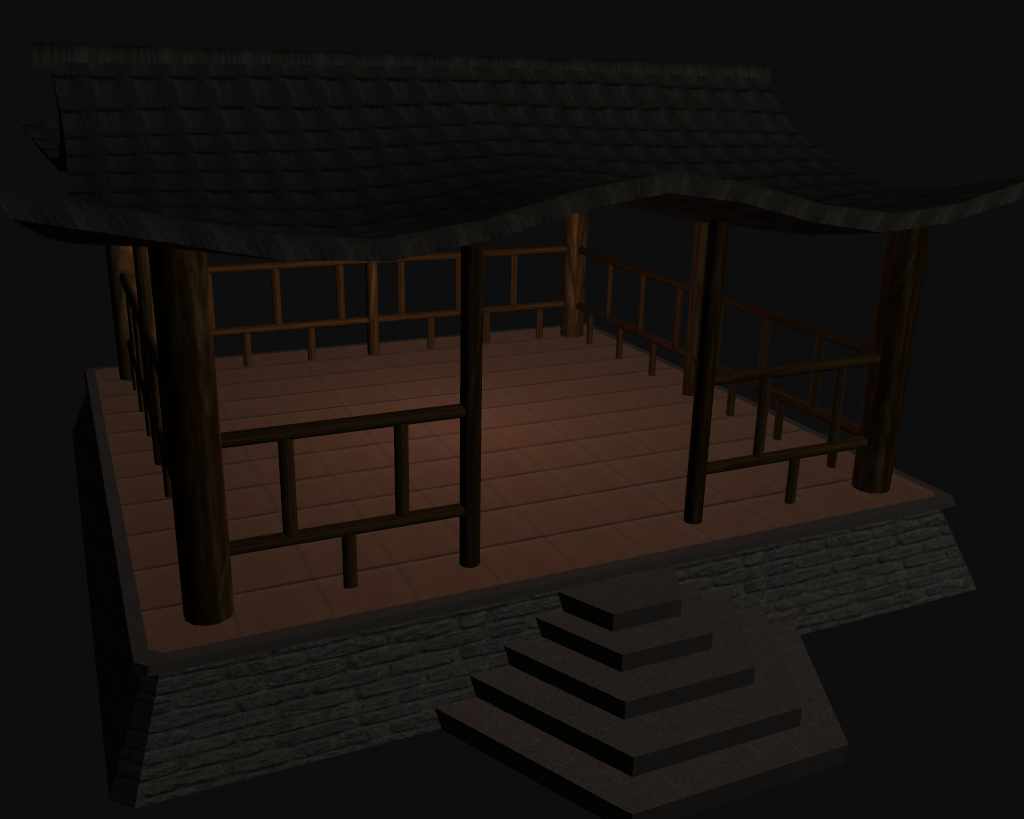
\includegraphics[width=2.2in]{rhan_shrine_1_per_pixel_lighting}
  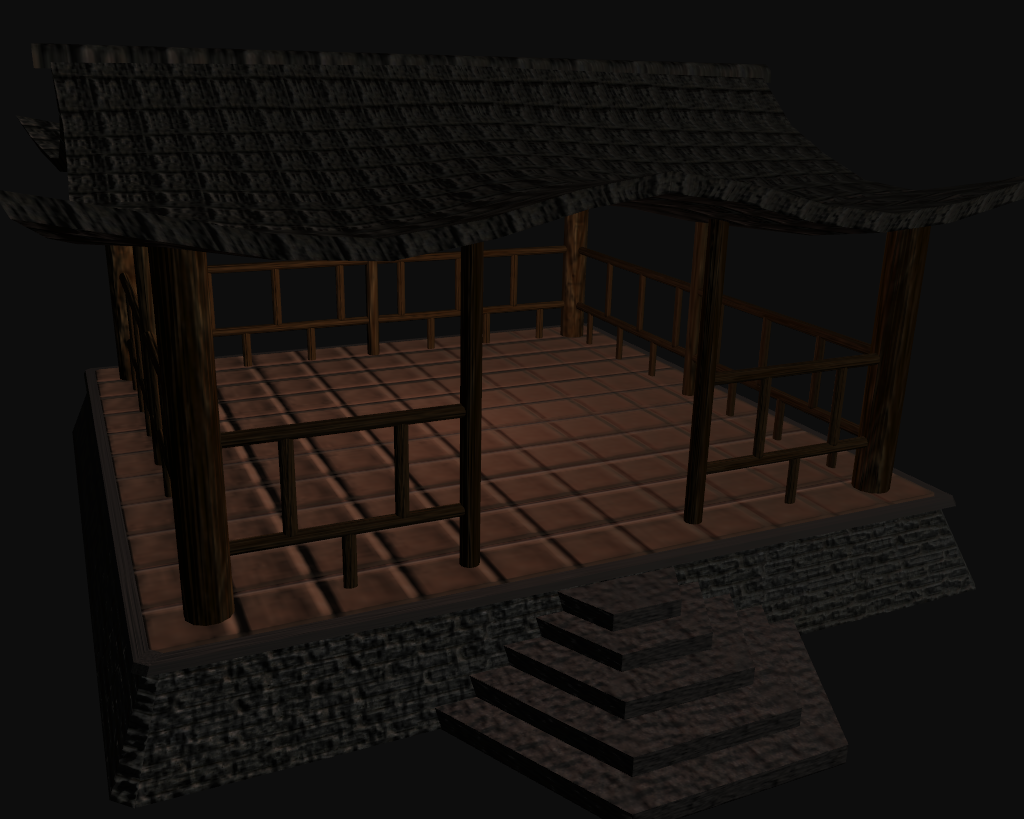
\includegraphics[width=2.2in]{rhan_shrine_2_bump_mapping}
  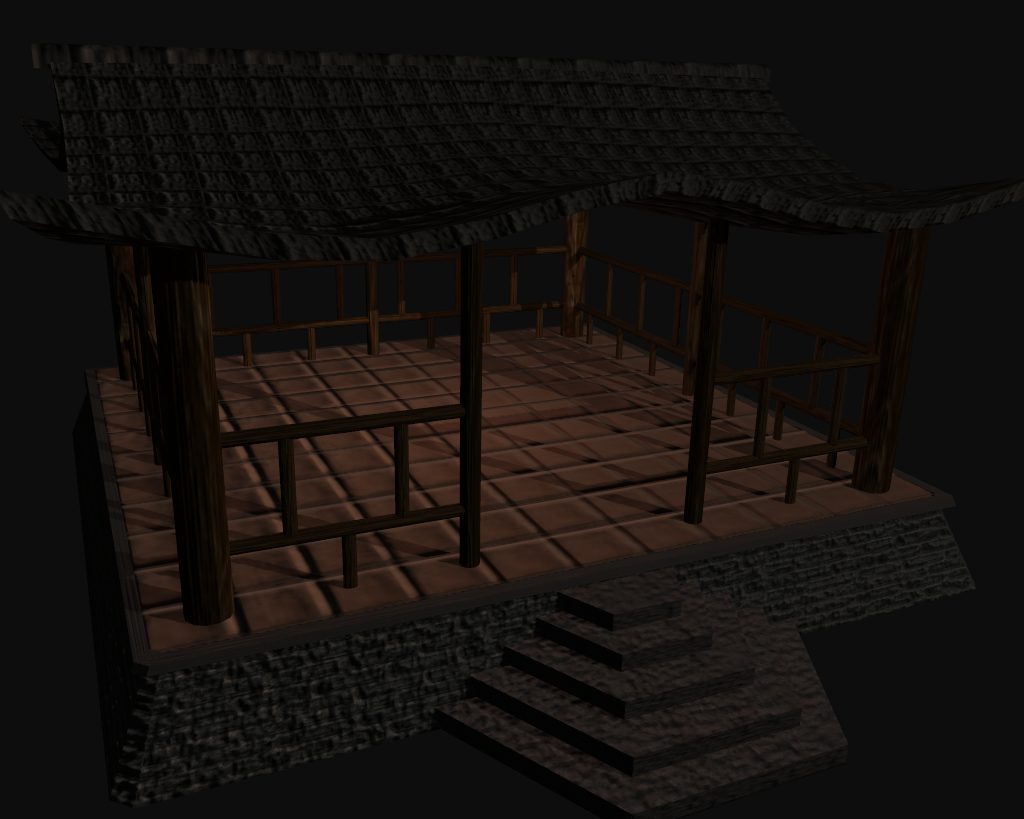
\includegraphics[width=2.2in]{rhan_shrine_3_shadow_1st}
  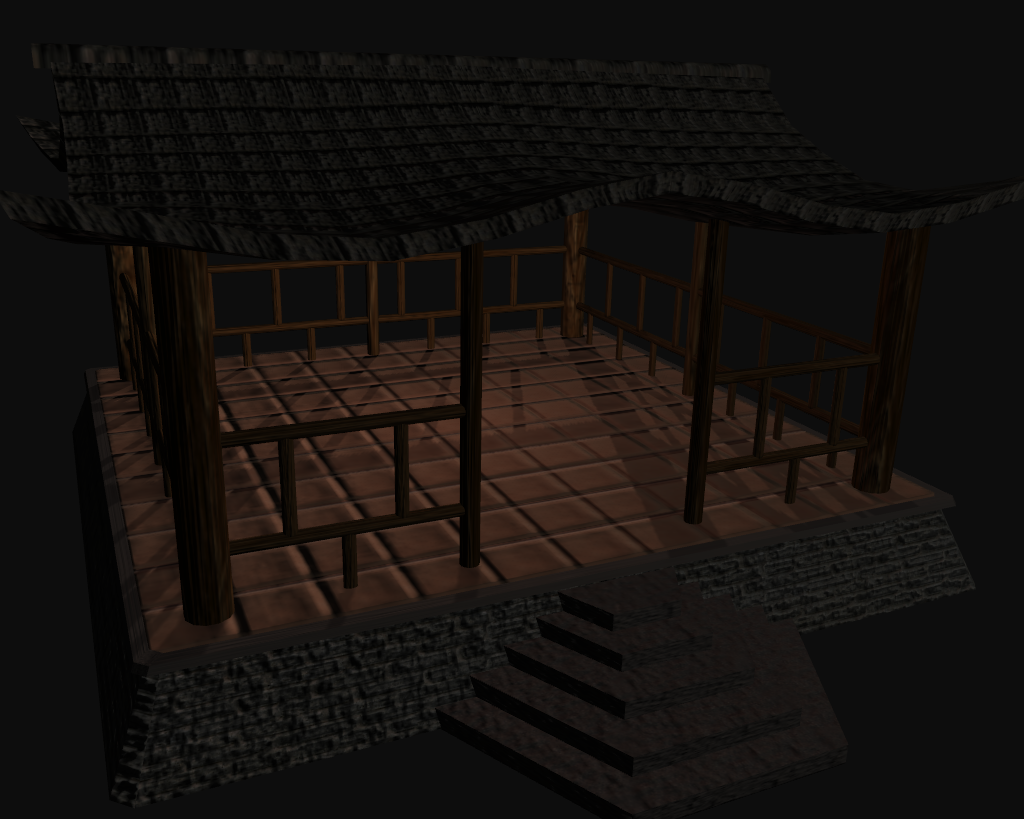
\includegraphics[width=2.2in]{rhan_shrine_4_shadow_2nd}
  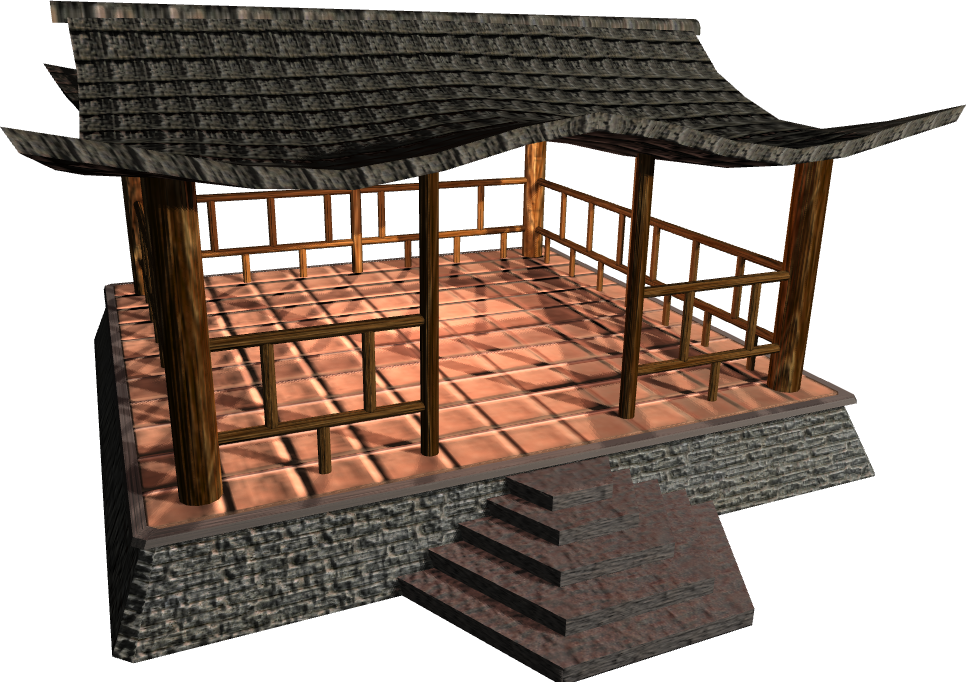
\includegraphics[width=2.2in]{rhan_shrine_5_everything}
  \caption{Japanese shrine model with more and more effects applied: Gouraud shading,
Phong shading (per-pixel lighting), bump mapping, shadows from 1st light,
shadows from 2nd light, shadows from both lights.}
%%  \label{fig_xxx}
\end{figure*}

\section{Plugging}

The basic idea of our approach is that a shader source code defines
a points when a calls to user-defined functions may be inserted. The mechanism
allows very easily to define new plugging points, and to use
them. Moreover, user shaders and browser internal shaders have the
same means to define and use plug points. This allows to connect
shaders (both user and browser) in a variety of ways.

A trivial example of an effect that makes colors two times brighter
follows. This is written in X3D classic encoding,
you should add this inside any \texttt{Appearance} node:

\begin{Verbatim}[commandchars=\\\{\},frame=single]
effects Effect \{
  language "GLSL"
  parts EffectPart \{
    type "FRAGMENT"
    url "data:text/plain,

\textbf{    void PLUG_texture_apply(}
\textbf{      inout vec4 fragment_color)}
\textbf{    \{}
\textbf{      fragment_color.rgb *= 2.0;}
\textbf{    \}}"
  \}
\}
\end{Verbatim}

It defines a GLSL function named \texttt{PLUG\_texture\_apply}
within an \texttt{EffectPart} node. Function names starting with \texttt{PLUG\_}
are special, they enhance some standard shader calculation. In particular
the \texttt{PLUG\_texture\_apply} is used after the normal texture colors are applied,
but before the alpha test, and is a usual place to ,,just modify the pixel color''.
\texttt{fragment\_color} is an \texttt{inout} parameter, by modifying it
you modify the color that will be displayed on screen (and the alpha that will
be tested).

We have a short reference (at the end of this document) of all
the plugging points available in our shaders. For each plugging point,
like this \texttt{PLUG\_texture\_apply}, we define a list of it's parameters
(you have to declare them exactly the same in your code), and we define
when it is called.

Various ways of defining and using ,,pluggins points'' (which we'll just call
,,plugs'' from now on) are possible:

\begin{myenumerate}
\itemsep 0pt
\item Browser shaders can be connected with each other. For example, we
have a basic shader code that defines lighting and texturing. Our bump
mapping is implemented by simply plugging the code in the appropriate
places in this base shader. This way, the base shader is completely
independent from the bump mapping implementation. We can switch bump
mapping implementations (for example, use bump texture from image or
some random noise) without trouble.

So even inside the engine, this allows for much easier shader generator.

\item User shaders may plug into browser shaders. This is the most usual
case. Our shaders define various points when you can plug your code,
and override or enhance our shading.

\item User shaders may also plug into another user shaders. User shaders
can trivially (by just adding a "magic" comment) define new plugging
points, which are usable by other user shaders. User effects can
define plugging points, which are available to the following effects
on the Appearance.effects list.

\end{myenumerate}

We allow user shaders (defined in the \texttt{ComposedShader} and such nodes) to
define additional plugging points. User shaders can use our plug names
(and thus work with the same effects), or they can invent their
own. They can also always add new plug points.

When you don't use an explicit shader (like \texttt{ComposedShader} node),
browser uses it's own internal basic shader. This shader is then
extended by effects like bump mapping (coming from internal browser
implementation), or by user effects. But you can also define your own
\texttt{ComposedShader} node. Then your own shader is enhanced by the
browser. TODO: ? If you define the same (or compatible) plugging
points, then the browser effects will be even added to your own
shader. And of course user effects are added to your shader.

In summary, the system works regardless if you use or not an explicit
shader on \texttt{Appearance.shaders} list.

\subsection{Effect node}

In the X3D file we add a field

\begin{mycode}
\underline{Appearance}
\begin{Verbatim}[commandchars=\\\{\}]
MFNode [] \codeem{effects} [] # Effect
\end{Verbatim}
\end{mycode}

that can hold any number of

\begin{mycode}
\underline{Effect : X3DNode}
\begin{Verbatim}[commandchars=\\\{\}]
SFString [] \codeem{language} ""
  # just like ComposedShader.language.
  # Will be used only for matching language shaders.
MFNode [] \codeem{parts} [] # EffectPart
  ... any number of fields,
      that will be passed
      as uniform to the shader,
      just like for ComposedShader node ...
\end{Verbatim}
\end{mycode}

\begin{mycode}
\underline{EffectPart : X3DNode, X3DUrlObject}
\begin{Verbatim}[commandchars=\\\{\}]
SFString [] \codeem{type} "VERTEX"
  # Allowed values like ShaderPart.type,
  # FRAGMENT | VERTEX | (once supported) GEOMETRY.
MFString [] \codeem{url} ""
  # source code, in external file (url),
  # or inline (following data:text/plain,).
  # Source code may also be inline in CDATA
  # in XML encoding,
  # exactly like standard ShaderPart.
\end{Verbatim}
\end{mycode}

The functions you want to override are automatically detected by names
starting like \texttt{PLUG\_}.

In a single \texttt{EffectPart} node, you can define many \texttt{PLUG\_}
functions. However, you can only plug functions into the declared shader
type. For example, you cannot plug into \texttt{texture\_apply} when
your type is \texttt{VERTEX}.
If your effect requires some processing per-vertex and some per-fragment,
you will probably use two \texttt{EffectPart} nodes, with appropriate types.
While this may seem like an arbitrary limitation,
this reflects how shader parts are declared in shading languages with
separate namespaces for vertex and fragment parts (like GLSL).
A single part may declare variables (uniform, varying and such),
and many functions that use them. But it must be completely within
one shader type.

At one point we tried the approach
to not look at any special function names in GLSL code,
and instead define a plug name in the separate field of the \texttt{EffectPart}
node. However this produced ugly code --- you had to split your algorithm
into many \texttt{EffectPart} nodes, each often containing only 1 or 2 lines
of code. Especially bad was the fact that you had to declare uniform variables
in a separate effect part, which in turn means that we cannot place
your effects parts in separate namespaces (like a compilation unit in GLSL),
which in turn makes the usage less secure.
Detecting \texttt{PLUG\_} function names in GLSL code is very easy,
and turned out to be the cleaner solution.

In case of shading languages that have separate compilation units
(like OpenGL shading language) the implementation may choose to place
each effect part in such separate unit. This allows for cleaner error detection
(as the parsing errors in effect code will not cause errors elsewhere,
and error messages will refer to line numbers in actual user code).
This also allows some namespace separation. For example, uniforms defined in one
effect part may not be visible in the other part, as they should be placed
in a separate namespace (like a separate compilation unit for GLSL) if possible.

All the effects on this list (with suitable language, and with
plugging points defined by the browser shader, or active shader on
\texttt{Appearance.shaders} list) will be used. Note that this is contrary to
the \texttt{Appearance.shaders}, which chooses only one shader.
For effects, we choose all of them (that are suitable).

\needspace{1in}
The most basic idea of this paper is to allow one to define two
independent shader effects, and then seamlessly connect them by simply
placing them both on \texttt{Appearance.effects} list. This also allows to
define a library of effects, that can be composited without any work
needed by user.

\begin{figure}[H]
  \centering
  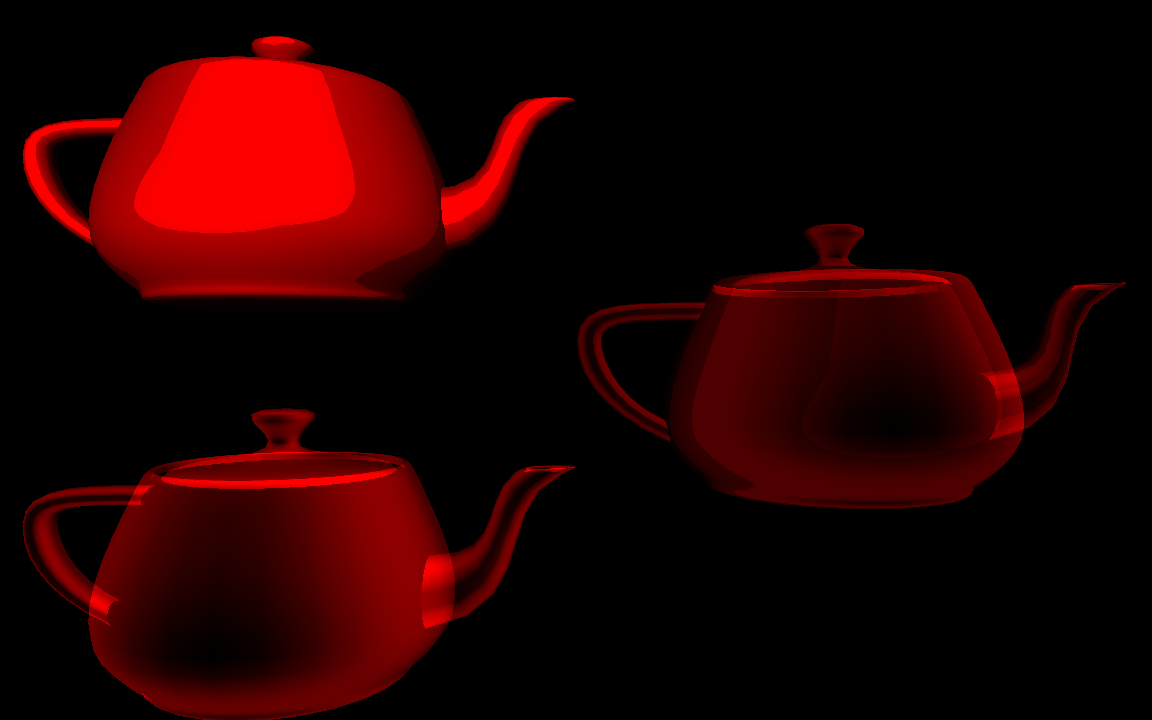
\includegraphics[width=3in]{fresnel_and_toon}
  \caption{Toon and Fresnel effects combined.}
\end{figure}

\subsection{Plugging from other nodes}

The real power of our system comes from the fact that some nodes,
like light sources, textures, or even fog, can define their own effects.
So you can easily define a shader specific for a given light source,
or texture. For this, we add the \texttt{effects} field to various nodes:

\begin{mycode}
\underline{X3DLightSource, X3DTextureNode, X3DFogObject}
\begin{Verbatim}[commandchars=\\\{\}]
MFNode [] \codeem{effects} [] # Effect
\end{Verbatim}
\end{mycode}

%% TODO check and fix above X3Dxxx class names.

You can modify the light source contribution, or even replace the default
calculation of light source contribution. In the second case,
the default calculation will not even be used in the shader,
so it will not slow down the calculation without a reason.

\subsection{Shader texture}

Although you can define plugs at any texture node, sometimes you just
want to define a texture contents completely by shaders. This means
that the texture contents are not stored anywhere (not even on GPU),
the X3D browser doesn't manage any texture resources and such.
From a GPU point of view, there is no texture\footnote{But the spoon is real,
we swear.}. There is only a shader function that generates colors
based on some vectors.

However it's still useful to let X3D ,,know'' that it is a texture.
This way we can generate automatic texture coordinates for the given
texture (using various methods supported by the
\texttt{TextureCoordinateGenerator} and \texttt{ProjectedTextureCoordinate}
nodes). For this reason, we introduce a new texture node:

\begin{mycode}
\underline{ShaderTexture : X3DTextureNode}
\begin{Verbatim}[commandchars=\\\{\}]
MFNode [] \codeem{effects} [] # Effect
\end{Verbatim}
\end{mycode}

(Actually, \texttt{effects} field is already defined at \texttt{X3DTextureNode},
see above. So in reality, \texttt{ShaderTexture} is just equal to
\texttt{X3DTextureNode}. We simply allow actually using it in X3D files,
while \texttt{X3DTextureNode} is left defined as an abstract class.)

You have to include an effect overriding at least the \texttt{texture\_color}
plug, otherwise texture contents are undefined.

\section{Defining your own plug points}

When you write shader code, you can define your own plug points by a
magic comment:

\begin{mycode}
/* PLUG: plug-name (param) (const in vec3 foo, inout vec4 bar) */
\end{mycode}

This defines a point when multiple user plugs may be added. Each
Effect with name matching given plug-name will cause a
definition of a new function, with the declaration as given above
(with \%s replaced by the automatic function name). This function will
be called at given place.

This is often useful for processing some parameter
repeatedly (like adding or modulating the fragment color),
so there's usually an inout parameter.

Special plug names \$declare-variables\$, \$declare-procedures\$
are used to designate a place where functions are placed.
May be specified within an effect part or ShaderPart within
your own ComposedShader node. It will be used to place
declarations (external declarations of functions in other compilation
units) at this point. Otherwise, they will be simply added to
the beginning of given part. TODO: this ,,otherwise'' is not yet impl,
and the treatment is hacky.

Multiple code pieces may be added to the given plug point.
So multiple effects may use the same plug point. They are added
in the order they are specified in the Appearance.effects list
(although, preferably, for most effects this order will not matter).

When a special value \texttt{function} is specified, like

\begin{mycode}
/* PLUG: plug-name function type-name (params-called) (params-declared) */
\end{mycode}

then the code will be replaced to a function call returning given type-name.
Such plug can only be used once.
Identifier (next token in GLSL language) immediately following
this plug will be removed if this plug is defined.
TODO: I'm unsure about the ,,function'' plugs.
I don't like the fact that they can only be used once, but sometimes
it really makes sense?
I'm also unsure about definition --- this may force authors to use
intermediate functions. Instead use closing /* PLUG-END: plug-name */?

\subsection{Why plugs are defined as comments}

The nice feature of our magic /* PLUG ... */ comments is that a shader source
is still valid even if you completely ignore the plugs. For example,
you can write your custom ComposedShader node, defining some plugs,
and for browsers that understand them --- the plugs can be used,
for other browsers --- plugs will be gracefully ignored (but still
the shader will run, although without any effects).

\subsection{More about defining plugs}

You can define the same plug name many times. In this case,
all occurrences of this plug will be appropriately replaced.

You can define plug points both inside your custom ComposedShader code,
as in the ,,effects'' code. In the latter case, the plug points
are only available for the following effects of the same node.

\subsection{Invalid shader code}

We guarantee the behavior only if the provided shading language code
is a correct, self-contained code.
X3D browser doesn't validate code in any way, so any error (like undeclared
variable, like unterminated block (,,{'' without matching ,,}''),
like unterminated comment) may be only detected after the complete shader
is determined and compiled by the GPU.

Although in case of shading languages with separate compilation units,
the separation is actually better, and parsing errors will cause
problems in your own code only. Still, by writing incorrect code,
you can cause the whole shader to malfunction.

In all our practical cases, this didn't cause any problems.
Since you code each effect separately, you also test them separately,
and in practice it's usually obvious what problem causes the parsing error.
This is also a direct consequence of our decision to \textbf{never require
the browser to parse the shader code}.

It should be noted however that in particularly nasty cases,
a deliberately poorly coded effect may cause troubles for other effects.
In particular, since you can use \#define and macros in your effect code,
you can do nasty tricks to break other effects. You can make them compile,
but function incorrectly. However, we don't consider
it a real problem. You really have to deliberately want to do something bad,
and often use an internal knowledge, to achieve something bad.
It doesn't happen by accident in our experience.
%% And you may need to use the internal knowledge
%% how the other effects are implemented (maybe how they are implemented
%% inside the browser).

Note that this isn't a security problem --- bad shader code only breaks
rendering of a particular shape. And X3D ComposedShader node allows users
to execute any shading language code anyway. So if there's anything dangerous,
you could do it without using our effects framework anyway.

\section{Usage examples}

Remember that effects may define their own uniform variables,
just like normal shader node. So you can pass your own textures
to effects. For example you can write an effect that mixes a couple of textures,
using any information available in the shader as a criteria for mixing.
You can also pass any other values for an effect, for example you can
pass the current time from a \texttt{TimeSensor} and make dynamic effects.

\begin{figure}[H]
  \centering
  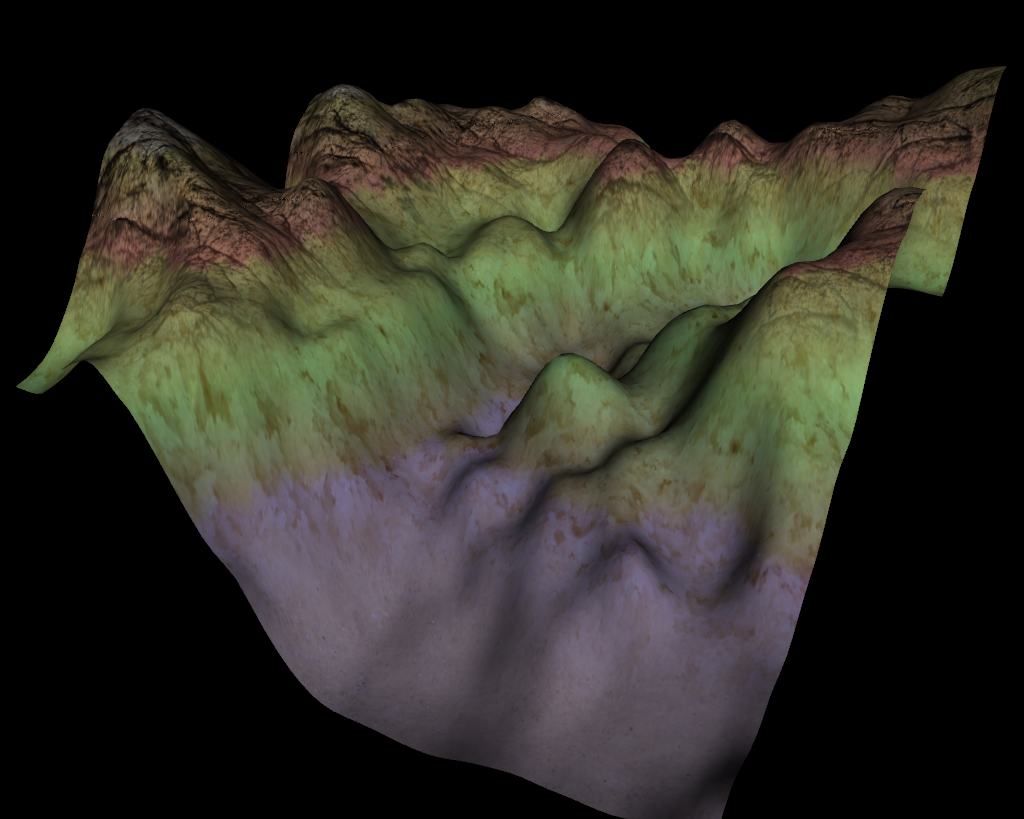
\includegraphics[width=3in]{terrain}
  \caption{ElevationGrid with 3 textures mixed based on height by GLSL effect.}
\end{figure}

An example effect for a light source is to use a fancy shape and equation
for light's spot.

\begin{figure}[H]
  \centering
  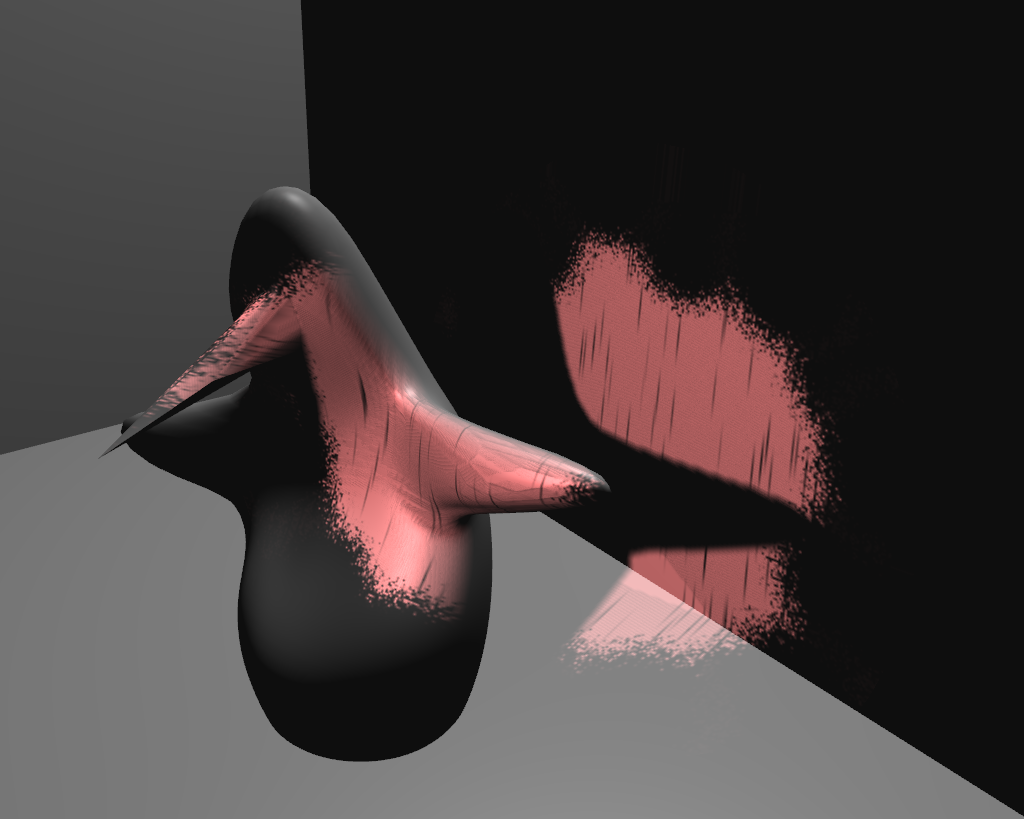
\includegraphics[width=3in]{fancy_light_spot_shape}
  \caption{Textured spot light with shadow.}
\end{figure}

Even inside the browse implementation, using plugs to implement internal
effects allows for a great code simplication and separation.
Our bump mapping effect (TODO: on slides, actually show
the trivial TVRMLShader.EnableBumpMapping source code?)
is done purely by using plugs.
So it has a clean and short implementation. It also shows that
X3D authors could implement perfect bump mapping themselves,
without any traditional hassles. For example, bump mapping can be
achieved using standard \texttt{ComposedShader} as well,
but then you have to write all this ,,boilerplate'' code to also deal
with all the possible lighting and textures configurations.
Well, the browser is still useful to calculate nice tangent vectors,
although an authoring program could generate GLSL attributes for them as well.

Same thing with shadow maps, they only plug to the \texttt{light\_scale}
calculation of appropriate light.

- Example how to implement some non-trivial effects:
  - water by plugs
  - fog / smoke?
  - grass moving under the wind

\section{Short reference of available plugs}

TODO: maybe make it a table? We can probably waste 0.5-1 page on this
without a problem. Document this at the end, when everything is settled down.

For each plug:
- plug name
- declaration (parameter order and types must match)
- type (fragment or vertex)
- docs: called when?

\section{Complete example models}

Examples are available inside our engine example models on
\myhref{http://vrmlengine.sourceforge.net/kambi\_vrml\_test\_suite.php}{http://vrmlengine.sourceforge.net/kambi_vrml_test_suite.php}.
You can checkout them from SVN, or just browse through a web browser,
using the URL
\myhref{https://vrmlengine.svn.sourceforge.net/svnroot/vrmlengine/trunk/kambi\_vrml\_test\_suite/compositing\_shaders/}{https://vrmlengine.svn.sourceforge.net/svnroot/vrmlengine/trunk/kambi_vrml_test_suite/compositing_shaders/}.
You can open them using any of our engine tools,
like \texttt{view3dscene} from
\myhref{http://vrmlengine.sourceforge.net/view3dscene.php}{http://vrmlengine.sourceforge.net/view3dscene.php}.

You can run \texttt{view3dscene} with \texttt{--debug-log} command-line
option. Output (stdout) will show you the final shader code generated.
This is a useful way to learn about our shader rendering internals.

Development notes: only the SVN kambi\_vrml\_test\_suite contains
compositing\_shaders subdirectory.
You also have to use view3dscene from SVN or nightly builds,
see \myhref{http://michalis.ii.uni.wroc.pl/vrmlengine-snapshots/}{http://michalis.ii.uni.wroc.pl/vrmlengine-snapshots/}.
And you have to activate ,,View $->$ Force Shader Rendering'' (Ctrl+S) manually.

\bibliographystyle{acmsiggraph}
\nocite{*}
\bibliography{compositing_shaders}

\end{document}
